\documentclass{beamer}

\newcommand{\lesson}{Binary Search Trees}


\newcommand{\course}{Introduction to Object-Oriented Programming}
\subject{\course}
\title[\lesson]{\course}
\subtitle{\lesson}

\author[CS 1331]
{Christopher Simpkins \\\texttt{chris.simpkins@gatech.edu}}
\institute[Georgia Tech]

\date[]{}

\newcommand{\link}[2]{\href{#1}{\textcolor{blue}{\underline{#2}}}}
\newcommand{\code}{http://cs1331.gatech.edu/code}

\usepackage{colortbl}

% If you have a file called "university-logo-filename.xxx", where xxx
% is a graphic format that can be processed by latex or pdflatex,
% resp., then you can add a logo as follows:

% \pgfdeclareimage[width=0.6in]{coc-logo}{cc_2012_logo}
% \logo{\pgfuseimage{coc-logo}}

\mode<presentation>
{
  \usetheme{Berlin}
  \useoutertheme{infolines}

  % or ...

 \setbeamercovered{transparent}
  % or whatever (possibly just delete it)
}

\usepackage{tikz}
% Optional PGF libraries
\usepackage{pgflibraryarrows}
\usepackage{pgflibrarysnakes}
\usepackage{pgfplots}
\usepackage{fancybox}
\usepackage{listings}
\usepackage{hyperref}
\hypersetup{colorlinks=true,urlcolor=blue}
\usepackage[english]{babel}
% or whatever

\usepackage[latin1]{inputenc}
% or whatever

\usepackage{times}
\usepackage[T1]{fontenc}
% Or whatever. Note that the encoding and the font should match. If T1
% does not look nice, try deleting the line with the fontenc.


\usepackage{listings}

% "define" Scala
\lstdefinelanguage{scala}{
  morekeywords={abstract,case,catch,class,def,%
    do,else,extends,false,final,finally,%
    for,if,implicit,import,match,mixin,%
    new,null,object,override,package,%
    private,protected,requires,return,sealed,%
    super,this,throw,trait,true,try,%
    type,val,var,while,with,yield},
  otherkeywords={=>,<-,<\%,<:,>:,\#,@},
  sensitive=true,
  morecomment=[l]{//},
  morecomment=[n]{/*}{*/},
  morestring=[b]",
  morestring=[b]',
  morestring=[b]""",
}

\usepackage{color}
\definecolor{dkgreen}{rgb}{0,0.6,0}
\definecolor{gray}{rgb}{0.5,0.5,0.5}
\definecolor{mauve}{rgb}{0.58,0,0.82}

% Default settings for code listings
\lstset{frame=tb,
  language=scala,
  aboveskip=2mm,
  belowskip=2mm,
  showstringspaces=false,
  columns=flexible,
  basicstyle={\scriptsize\ttfamily},
  numbers=none,
  numberstyle=\tiny\color{gray},
  keywordstyle=\color{blue},
  commentstyle=\color{dkgreen},
  stringstyle=\color{mauve},
  frame=single,
  breaklines=true,
  breakatwhitespace=true,
  keepspaces=true
  %tabsize=3
}


\usepackage{qtree}

\beamerdefaultoverlayspecification{<+->}


\begin{document}

\begin{frame}
  \titlepage
\end{frame}

%------------------------------------------------------------------------
\begin{frame}[fragile]{}

Trees are everywhere.

\begin{center}
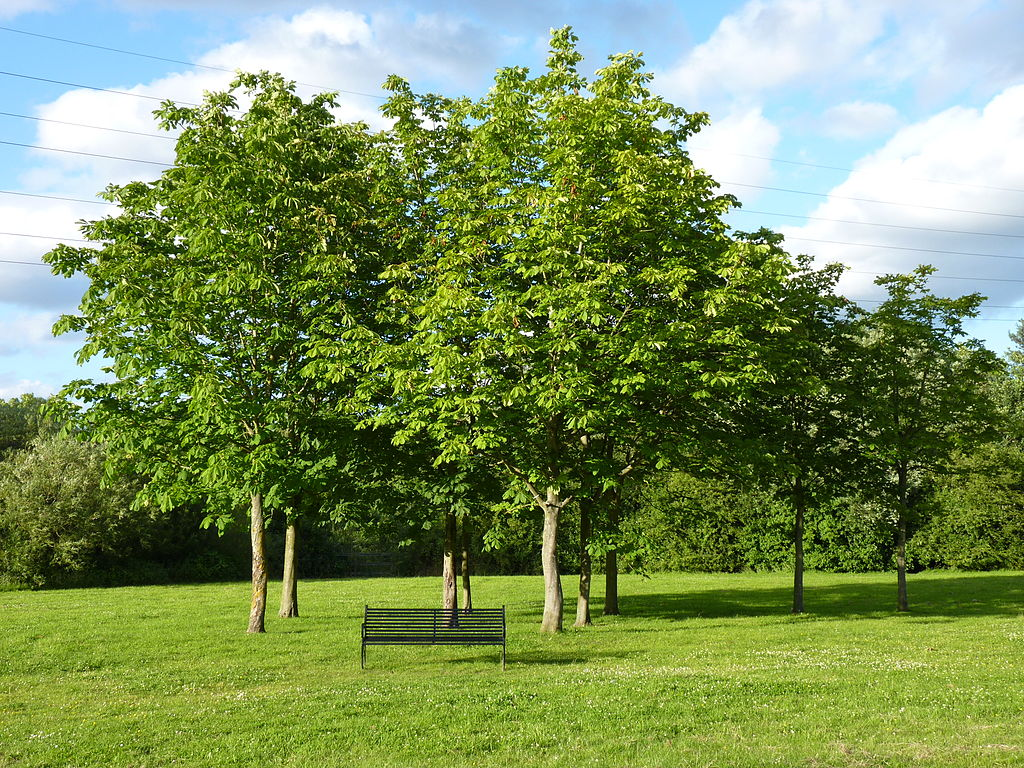
\includegraphics[height=2.5in]{1024px-Winnersh_Meadows_Trees.jpg}\footnote{Source:\url{ http://commons.wikimedia.org/wiki/File:Winnersh_Meadows_Trees.jpg}}
\end{center}

\end{frame}
%------------------------------------------------------------------------

%------------------------------------------------------------------------
\begin{frame}[fragile]{}

They're in our web browsers.

\begin{center}
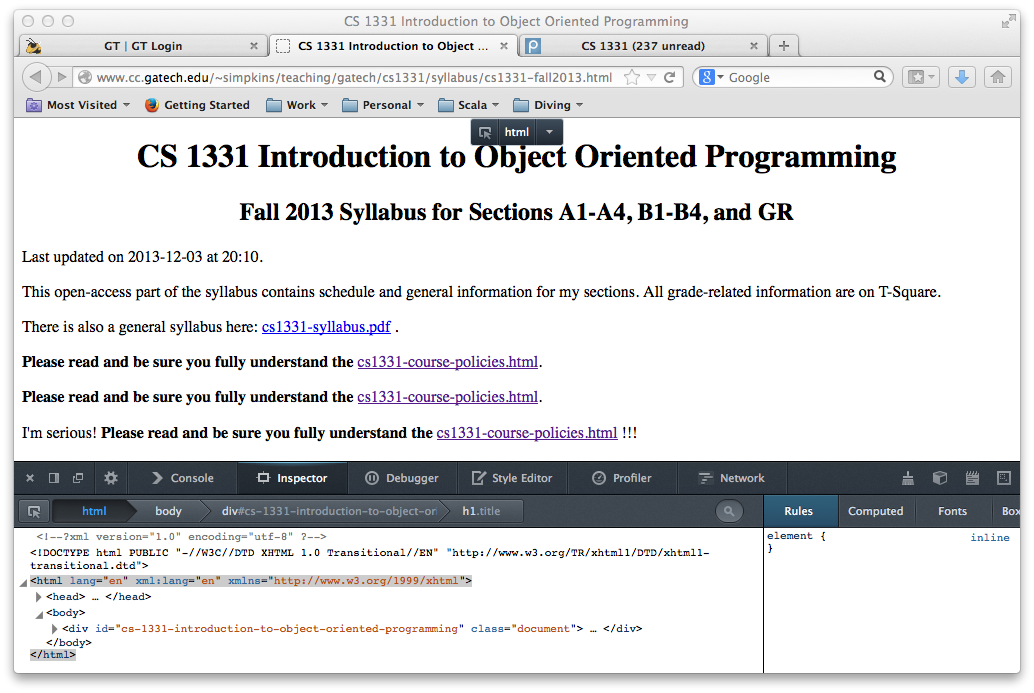
\includegraphics[height=3in]{xhtml-tree.png}
\end{center}

\end{frame}
%------------------------------------------------------------------------

%------------------------------------------------------------------------
\begin{frame}[fragile]{}

They're in our file systems.

\begin{center}
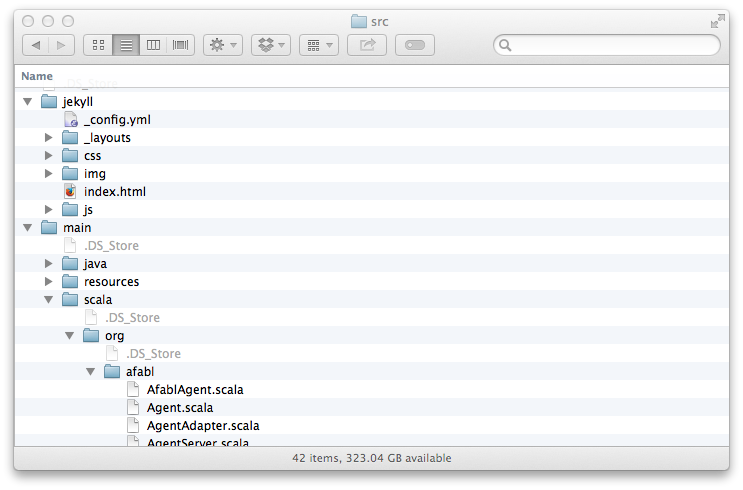
\includegraphics[height=3in]{directory-tree.png}
\end{center}

\end{frame}
%------------------------------------------------------------------------


%------------------------------------------------------------------------
\begin{frame}[fragile]{}

They're even in pop culture.

\begin{center}

\includegraphics[height=2.5in]{Neon+Trees.png}\footnote{Source: \url{http://userserve-ak.last.fm/serve/500/44019065/Neon+Trees.png}}
\end{center}

\end{frame}
%------------------------------------------------------------------------

%------------------------------------------------------------------------
\begin{frame}[fragile]{}

But they're not in Kansas.

\begin{center}
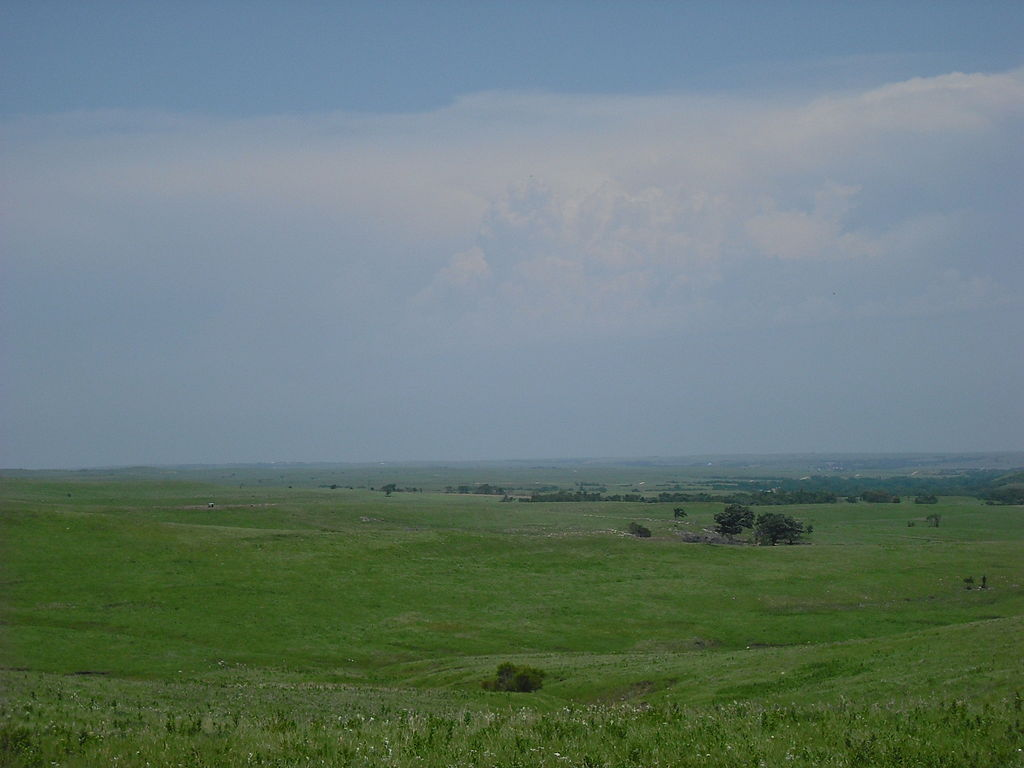
\includegraphics[height=2.5in]{1024px-Wabaunsee_County_View.JPG}\footnote{Source: \url{http://en.wikipedia.org/wiki/File:Wabaunsee_County_View.JPG}}
\end{center}

\end{frame}
%------------------------------------------------------------------------


%------------------------------------------------------------------------
\begin{frame}[fragile]{Binary Tree Nodes}


The nodes of a binary tree have
\begin{itemize}
\item a data item,
\item a link to a left node, and
\item a link to a right node.
\end{itemize}

\begin{lstlisting}[language=Java]
    private class Node<E> {
        E item;
        Node<E> left;
        Node<E> right;

        Node(E item, Node<E> left, Node<E> right) {
            this.item = item;
            this.left = left;
            this.right = right;
        }
    }
\end{lstlisting}

Just as in the other linked data structures we've studied, binary trees are recursive.


\end{frame}
%------------------------------------------------------------------------

%------------------------------------------------------------------------
\begin{frame}[fragile]{Binary Tree Structure}

\begin{itemize}
\item Every tree has a distinguished {\it root node} with no parent.
\begin{itemize}
\item All other nodes have exactly one parent.
\end{itemize}
\item Nodes which have no children are called {\it leaf nodes}.
\item Nodes which have children are called {\it interior nodes}.
\item Every node has 0, 1, or 2 children.
\item Every node can be reached by a unique path from the root node.
\end{itemize}

\begin{center}
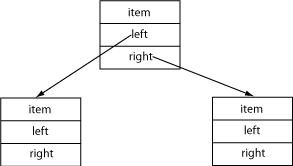
\includegraphics[height=1.25in]{binary-tree.png}
\end{center}


\end{frame}
%------------------------------------------------------------------------

%------------------------------------------------------------------------
\begin{frame}[fragile]{Binary Search Trees}


A binary search tree (BST) encodes the binary search algorithm into its
structure.  The BST property: for any node,
\begin{itemize}
\item all the elements in the node's left subtree are less than the node's data item, and
\item all the elements in the node's right subtree are equal to or greater than the node's data item.
\end{itemize}

A BST is distinguished by this property, but it's ADT is just like the others we've seen: add elements, find element's in the tree, and iterate over the elements in a tree.


\end{frame}
%------------------------------------------------------------------------

%------------------------------------------------------------------------
\begin{frame}[fragile]{Maintaining The BST Property}

To add a new value to binary tree and maintain the BST property, we
\begin{itemize}
\item insert new nodes for data items into the left subtree of a node if the new item is less than the node's item, or
\item the right subtree otherwise.
\end{itemize}
Every new item creates a leaf node, which can later become an interior node after additional items have been added. Here's the structure of a BST after adding the sequence of numbers 3, 4, 1, 5, 2:
\vspace{-.05in}
\begin{center}
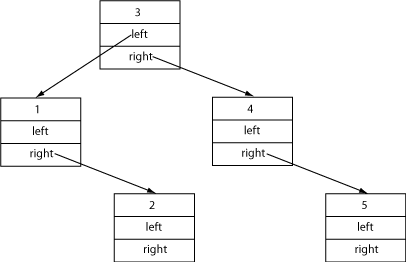
\includegraphics[height=1.5in]{binary-tree-nums.png}
\end{center}

\end{frame}
%------------------------------------------------------------------------

%------------------------------------------------------------------------
\begin{frame}[fragile]{Adding Elements to a BST}

\begin{lstlisting}[language=Java]
public class BinarySearchTree<E extends Comparable<? super E>>
        implements Iterable<E> {

    protected class Node<E> { ... }

    protected Node<E> root;

    public void add(E item) {
        root = insert(item, root);
    }
    protected Node<E> insert(E newItem, Node<E> node) {
        if (node == null) {
            return new Node<E>(newItem, null, null);
        } else if (newItem.compareTo(node.item) < 0) {
            node.left = insert(newItem, node.left);
            return node;
        } else {
            node.right = insert(newItem, node.right);
            return node;
        }
    }
\end{lstlisting}


\end{frame}
%------------------------------------------------------------------------

%------------------------------------------------------------------------
\begin{frame}[fragile]{Exercise: Insertion Locations}


Given the following tree that conforms to the binary search tree property:\\

\Tree [.6 [.3 1 5 ] [.9 7 [.11 10 15 ] ] ]

\vspace{.25in}

Where would 2, 4, 8, and 16 be inserted in the tree?

\end{frame}
%------------------------------------------------------------------------


%------------------------------------------------------------------------
\begin{frame}[fragile]{Traversing a Binary Tree}


There are three primary ways to traverse a binary tree:

Pre-order:
\begin{itemize}
\item Process node's item.
\item Process left subtree.
\item Process right subtree.
\end{itemize}

In-order:
\begin{itemize}
\item Process left subtree.
\item Process node's item.
\item Process right subtree.
\end{itemize}

Post-order:
\begin{itemize}
\item Process left subtree.
\item Process right subtree.
\item Process node's item.
\end{itemize}


\end{frame}
%------------------------------------------------------------------------

%------------------------------------------------------------------------
\begin{frame}[fragile]{Simple In-Order Traversal}

Traversal code follows the recursive structure of the tree:
\begin{lstlisting}[language=Java]
    public void printInOrder() {
        printInOrder(root);
    }

    private void printInOrder(Node<E> node) {
        if (node != null) {
            printInOrder(node.left);
            System.out.print(node.item + " ");
            printInOrder(node.right);
        }
    }
\end{lstlisting}
The code above prints the elements in ascending order.
Let's add a {\tt printDescending()} method to \link{\code/data-structures/BinarySearchTree.java}{BinarySearchTree.java}.

\end{frame}
%------------------------------------------------------------------------

%------------------------------------------------------------------------
\begin{frame}[fragile]{Exercise: Traversal Orders}

Given the following tree:\\

\Tree [.+ [.* 1 3 ] [.- 7 5 ] ]

\vspace{.2in}

If we proecssed each element by printing it, in what order would the elements be printed

\begin{itemize}
\item For a pre-order traversal:
\item For an in-order traversal:
\item For a post-order traversal:
\end{itemize}

\end{frame}
%------------------------------------------------------------------------

%------------------------------------------------------------------------
\begin{frame}[fragile]{The Path to an Item}

To find a path to an item in a BST:
\begin{itemize}
\item set the path to the empy list
\item set the root node as the currentNode
\item until we find the node containing the item or exhaust the BST:
\begin{itemize}
\item if currentNode contains the item, add it to the path and return it
\item else if query item is less than the item in currentNode, add currentNode to path and set the left child as the new currentNode
\item else add add currentNode to path and set the right child as the new currentNode
\end{itemize}
\item if the item wasn't found, set the path to the empty list
\end{itemize}


\end{frame}
%------------------------------------------------------------------------

%------------------------------------------------------------------------
\begin{frame}[fragile]{Path Examples}
\vspace{-.1in}
Adding the elements {\tt [3, 4, 1, 5, 2]} to a BST would result in the
following structure:

\Tree [.3 [.1 nil 2 ] [.4 nil [.5 nil nil ] ] ]

and the paths to each element in the tree would be:
\begin{itemize}
\item Path to 1: [3, 1]
\item Path to 2: [3, 1, 2]
\item Path to 3: [3]
\item Path to 4: [3, 4]
\item Path to 5: [3, 4, 5]
\end{itemize}

See {\tt public List<E> path(E queryItem)} in \link{\code/data-structures/BinarySearchTree.java}{BinarySearchTree.java} for the code.

\end{frame}
%------------------------------------------------------------------------

%------------------------------------------------------------------------
\begin{frame}[fragile]{Exercise: Paths}

Given the following tree:\\

\Tree [.8 [.4 [.2 1 3 ] [.6 5 7 ] ] [.12 [.10 9 11 ] [.14 13 15 ] ] ]

\vspace{.2in}

\begin{itemize}
\item What's the path to 1?
\item Whats the path to 11?
\end{itemize}


\end{frame}
%------------------------------------------------------------------------


%------------------------------------------------------------------------
\begin{frame}[fragile]{Recursively Building a Result: {\tt inOrderList()}}

We can use the recursive accumulator idiom to collect the elements of the tree in an in-order traversal:
\begin{lstlisting}[language=Java]
    public List<E> toList() {
        return inOrderList(root, new ArrayList<E>());
    }

    private List<E> inOrderList(Node<E> node, List<E> accum) {
        if (null == node) {
            return accum;
        } else {
            inOrderList(node.left, accum);
            accum.add(node.item);
            inOrderList(node.right, accum);
        }
        return accum;
    }
\end{lstlisting}

Again, the code follows the recursive structure of the tree.

\end{frame}
%------------------------------------------------------------------------

%------------------------------------------------------------------------
\begin{frame}[fragile]{Imperative traveral: {\tt inOrderImperative()}}
\vspace{-.05in}
Contrast the previous code for getting an in-order list of BST elements with an imperative version:
\vspace{-.05in}
\begin{lstlisting}[language=Java]
    public List<E> inOrderImperative() {
        Node<E> curNode = root;
        Stack<Node<E>> fringe = new LinkedStack<>();
        List<E> accum = new ArrayList<E>();
        while ((curNode != null) || !fringe.isEmpty()) {
            while (curNode != null) {
                fringe.push(curNode);
                curNode = curNode.left;
            }
            curNode = fringe.pop();
            accum.add(curNode.item);
            curNode = curNode.right;
        }
        return accum;
    }
\end{lstlisting}
\vspace{-.05in}
We need extra bookkeeping variables to keep track of where we are in the tree so we can back-track.  See \link{\code/data-structures/BinarySearchTree.java}{BinarySearchTree.java} for comments explaining the algorithm.

\end{frame}
%------------------------------------------------------------------------


%------------------------------------------------------------------------
\begin{frame}[fragile]{Iterators}


Iterators can free clients from having to implement traversal algorithms.  We can even plug our data structures into Java's for-each loop by implementing {\tt java.lang.Iterable}:
\begin{lstlisting}[language=Java]
public interface Iterable<T> {
    java.util.Iterator<T> iterator();
}
\end{lstlisting}
As a reminder, {\tt java.util.Iterator}:
\begin{lstlisting}[language=Java]
public interface Iterator<E> {
    boolean hasNext();

    E next();

    void remove();
}
\end{lstlisting}

\end{frame}
%------------------------------------------------------------------------

%------------------------------------------------------------------------
\begin{frame}[fragile]{Stateful In-Order Tree Traversal}


In the traversal examples we saw earlier the traversal order was effected by the method call stack.  A stateful iterator is much more challenging because:

\begin{itemize}
\item The iterator must remember where it is in the tree
\item The iterator must be able to back-track to parent nodes after processing child branches
\end{itemize}

The essential implementation idea is to use a stack to store nodes for back-tracking.  Traditionally (at least in AI), this ``to-do list'' stack is called the {\it fringe}.

Let's look at \link{\code/data-structures/BinarySearchTree.java}{BinarySearchTree.java} again to see how we implement a stateful in-order iterator.

\end{frame}
%------------------------------------------------------------------------


%------------------------------------------------------------------------
\begin{frame}[fragile]{Analysis of BSTs}

What is the Big-O of finding an element in a BST?\\

\Tree [.8 [.4 [.2 1 3 ] [.6 5 7 ] ] [.12 [.10 9 11 ] [.14 13 [.15 nil 16 ] ] ] ]

\begin{itemize}
\item <2-> Proportional to height of tree
\item <3-> Height of tree is proportional to $\log n$
\item <4-> 16-element tree has height 4
\end{itemize}


\end{frame}
%------------------------------------------------------------------------

%------------------------------------------------------------------------
\begin{frame}[fragile]{Height of BST Proportional to $\log n$}


\Tree [.4 [.2 1 3 ] [.6 5 [.7 nil 8 ] ] ]

\vspace{.2in}

8-element tree has height 3

\end{frame}
%------------------------------------------------------------------------


%------------------------------------------------------------------------
\begin{frame}[fragile]{End of course cliff hanger ...}

What if we add elements to a BST in order?

\Tree [.1 nil [.2 nil [.3 nil [.4 nil [.5 nil 6 ] ] ] ] ]

\begin{itemize}
\item <2-> We end up with a linked list!
\item <3-> In your algorithms and data structures course you'll learn how to maintain a balanced binary search tree.
\end{itemize}

\end{frame}
%------------------------------------------------------------------------

% %------------------------------------------------------------------------
% \begin{frame}[fragile]{Programming Exercise 1}
%
% Add a {\tt toString} method to {\tt BinarySearchTree}.
% \begin{itemize}
% \item The string should have a left square bracket, followed by the elements in the BST in-oder separated by spaces, followed by a right square bracket.  For example, {\tt [1 2 3 4 ]}
% \item If the BST is empty, the string should contain empty square barckets, e.g., {\tt []}.
% \end{itemize}
% Your {\tt toString} method should use a recursive helper method, similar to {\tt inOrderList}.  Your helper method should use a {\tt StringBuilder} for its accumulator.  \footnote{{\tt StringBuilder} works just like {\tt StringBuffer}.  What's the difference?}
%
% \end{frame}
% %------------------------------------------------------------------------
%
% %------------------------------------------------------------------------
% \begin{frame}[fragile]{Programming Exercise 2}
%
% Recall the method that adds nodes to the {\tt BinarySearchTree}:
% \begin{language=Java}[language=Java]
%     private Node<E> insert(E newItem, Node<E> node) {
%         if (node == null) {
%             return new Node<E>(newItem, null, null);
%         } else if (newItem.compareTo(node.item) < 0) {
%             node.left = insert(newItem, node.left);
%             return node;
%         } else {
%             node.right = insert(newItem, node.right);
%             return node;
%         }
%     }
% \end{lstlisting}
% Notice that this implementation allows duplicate items.  Modify this method so that {\tt BinarySearchTree} is a set, that is, does not insert duplicate items.
%
%
% \end{frame}
% %------------------------------------------------------------------------
%


% %------------------------------------------------------------------------
% \begin{frame}[fragile]{}


% \begin{lstlisting}[language=Java]

% \end{lstlisting}

% \begin{itemize}
% \item
% \end{itemize}


% \end{frame}
% %------------------------------------------------------------------------


\end{document}
